% ----------------------------------------------------------------------------
\chapter{Implementation of the Prototype}
The prototype was developed using the spiral software development model.
It is named \textit{ceof}. The source code can be found in the 
directory \textit{src}.
% 5. Technical documentation and prototype for the new chat system
% ----------------------------------------------------------------------------
\section{Environment}
The prototype was developed using the Python3 programming language.
In addition to the standard libraries, the python-gnupg module is required.
To create a python environment that is suitable for running and developing
the prototype, a new virtualenv including the required python-gnupg module
can be created using the following commands:
\begin{verbatim}
% virtualenv -p /usr/bin/python3 python-env
% . ./python-env/bin/activate
% pip install python-gnupg
% (cd python-env/bin && ln -s python python3)
\end{verbatim}
Because python is an interpreted scripting language with interpreters
available for all major platforms, the prototype should be runnable
on all major platforms.
All configurations are saved in the \textit{cconfig}\cite{cconfig} format.
The path to the configuration directory is usually derived by taking
the content of the environment variable \textit{HOME} and appending
the subdirectory \textit{.ceof}. On Unix this is referenced as
\textit{\textasciitilde{}/.ceof/}.
% ----------------------------------------------------------------------------
\section{Usage}
% ----------------------------------------------------------------------------
\subsection{Command Line Interface (CLI)}
The implemented prototype provides a command line interface to access
all functionality.
All operations are grouped into commands, which are handled by the
executable \textit{bin/ceof}. If a subcommand is followed by the parameter
\textit{-h}, then a usage screen is displayed.
% ----------------------------------------------------------------------------
\subsection{Cryptographic Operations}
All cryptographic operations are accessible by using the \textit{crypto}
command, as shown in figure \ref{cryptohelp}.
This module uses the python-gnupg module for cryptographic functionality.
\begin{figure}[htbp]
\caption{Crypto Command Usage}
\label{cryptohelp}
\begin{verbatim}
(python-env)[18:40] brief:src% ./bin/ceof crypto -h
usage: ceof crypto [-h] [-d] [-v] [-c CONFIG_DIR]
                   [--encrypt ENCRYPT [ENCRYPT ...]] [--decrypt] [-e] [-f]
                   [-g] [-i] [-l LENGTH] [--name NAME]
                   [--email-address EMAIL_ADDRESS] [-s]

optional arguments:
  -h, --help            show this help message and exit
  -d, --debug           Set log level to debug
  -v, --verbose         Set log level to info, be more verbose
  -c CONFIG_DIR, --config-dir CONFIG_DIR
                        Select configuration directory ($HOME/.ceof by
                        default)
  --encrypt ENCRYPT [ENCRYPT ...]
                        Encrypt from stdin (specify recipients)
  --decrypt             Decrypt from stdin
  -e, --export          Export public key to stdout
  -f, --fingerprint     Show key fingerprint
  -g, --gen-key         Generate new private/public key pair
  -i, --import          Import public key from stdin
  -l LENGTH, --length LENGTH
                        Specify bit length for key generation
  --name NAME           Name (for key generate)
  --email-address EMAIL_ADDRESS
                        E-Mail-Address (for key generate)
  -s, --show            Show private/public key pair

Get ceof at http://www.nico.schottelius.org/software/ceof/
\end{verbatim}
\end{figure}
At first is it required to create a new public/private key pair using
the \textit{-{}-gen-key} parameter (figure \ref{genkey}), which can
be displayed using the \textit{-{}-show} parameter (figure \ref{showkey})
and exported using the \textit{-{}-export}
parameter (figure \ref{exportkey}).
\begin{figure}[htbp]
\caption{Generation of Public/Private Key Pair}
\label{genkey}
\begin{verbatim}
(python-env)[18:52] brief:src% ./bin/ceof crypto --gen-key 
    --name "Nico Schottelius" --email-address "nico@example.org"
\end{verbatim}
\end{figure}
\begin{figure}[htbp]
\caption{Show Public/Private Key Pair}
\label{showkey}
\begin{verbatim}
(python-env)[18:54] brief:src% ./bin/ceof crypto --show
{'dummy': '', 'keyid': 'C5FC26760DD842D6', 'expires': '', 'length': '2048',
'ownertrust': '', 'algo': '1',
'fingerprint': '77E54EF64A6395FF2769B2F4C5FC26760DD842D6',
'date': '1339174371', 'trust': '', 'type': 'sec',
'uids': ['Nico Schottelius (EOF42KEY) <nico@example.org>']}
\end{verbatim}
\end{figure}
\begin{figure}[htbp]
\caption{Export Public Key}
\label{exportkey}
\begin{verbatim}
(python-env)[19:23] brief:src% ./bin/ceof crypto --export
-----BEGIN PGP PUBLIC KEY BLOCK-----
Version: GnuPG v2.0.19 (GNU/Linux)

mQENBE/SLeMBCACu5sWt3j/ZTqZZ5eZw+cTvkIG6DwWaeVZjv+A+Dd7xZhbMBeyZ
q70CuOEURGLQUQQKtyT7bvTBjk8lkL2zcgIJ2a/MQQneJc+fEqB+ovlPM+Bl4qLf
TIuBMPnI+1OMOuTx0Agtys+6/9YaIdKaedtIqrZhVVsbaFAeE6MTHSm0i9bTtvyk
bH+X0JurCNL8nKEjf6SdSrQGdmohV/VyQTGlMZPaYG58LjCMKxbqWMb3lVKsmyRr
N4bZFPePzqBJzmqyH/noyoNuzbSUhNvUw27JzTL51u1JfMm2kQmkG1NZgLwXg6/W
e5FYbVoVI3LMj9NDABZ42y3mCv0QJJP6LkvdABEBAAG0Lk5pY28gU2Nob3R0ZWxp
dXMgKEVPRjQyS0VZKSA8bmljb0BleGFtcGxlLm9yZz6JATgEEwECACIFAk/SLeMC
Gy8GCwkIBwMCBhUIAgkKCwQWAgMBAh4BAheAAAoJEMX8JnYN2ELW8rcH/3Hdanzp
mUNfF7RqlU7sCwrGKFABOvTZtWQBfURLfTW2kMZRZEViRu6t3aB0hK3g1HWaSBzb
yXJmH6UznpkOG5gD+Y/FfMCiR7VZaiFXEZh9ukRWDwCytouoILdrey08Wr4YQEDf
+Ny38gLYu06Svnm25iQn3LiejTohCny5POkOnxfyVxOEhQ6LUjai6j0bSKk05o62
b2ZdKpGHsBqo9eHLr4y83JmoO5pSXDByBG0pu2Ukczey8BGuBwngUwEN/XKrl1xZ
aYHlpVNhCNsXthSAJdlag5Auju/t2S978yelO4Ii411dyDPrYZKjd4TGWbWfeVpS
jXOLmX++gs2tPyM=
=LB0W
-----END PGP PUBLIC KEY BLOCK-----
\end{verbatim}
\end{figure}
Importing keys is possible via standard input (\textit{stdin})
and shown in figure \ref{importkey}.
\begin{figure}[htbp]
\caption{Import Public Key}
\label{importkey}
\begin{verbatim}
# Export key from test peer0  and import into normal
# configuration directory
./bin/ceof crypto --config-dir ../test/peers/0 --export | 
    ./bin/ceof crypto --import
\end{verbatim}
\end{figure}
Furthermore de- and encryption are supported.
% -----------------------------------------------------------------------------
\subsection{Listener}
The \textit{listener} command is used
to configure to which addresses the prototype is listening to (figure
\ref{listenerusage}).
\begin{figure}[htbp]
\caption{Listener Command Usage}
\label{listenerusage}
\begin{verbatim}
(python-env)[18:41] brief:src% ./bin/ceof listener -h
usage: ceof listener [-h] [-d] [-v] [-c CONFIG_DIR] [-a ADD] [-l] [-r REMOVE]

optional arguments:
  -h, --help            show this help message and exit
  -d, --debug           Set log level to debug
  -v, --verbose         Set log level to info, be more verbose
  -c CONFIG_DIR, --config-dir CONFIG_DIR
                        Select configuration directory ($HOME/.ceof by
                        default)
  -a ADD, --add ADD     Add an address to listen on
  -l, --list            List listener
  -r REMOVE, --remove REMOVE
                        Remove an address to listen on

Get ceof at http://www.nico.schottelius.org/software/ceof/
\end{verbatim}
\end{figure}
For the initial setup it is required to configure at least one listener
using the \textit{-{}-add} parameter, which can be shown afterwards using
\textit{-{}-list} parameter (figure \ref{addandlistlistener}). 
Protection against adding unsupported addresses is included.
\begin{figure}[htbp][htb]
\caption{Add and list listener addresses}
\label{addandlistlistener}
\begin{verbatim}
(python-env)[19:23] brief:src% ./bin/ceof listener --list
(python-env)[19:42] brief:src% ./bin/ceof listener --add tcp://0.0.0.0:42507
(python-env)[19:42] brief:src% ./bin/ceof listener --add tcp://0.0.0.0:42508
(python-env)[19:42] brief:src% ./bin/ceof listener --list                   
tcp://0.0.0.0:42507
tcp://0.0.0.0:42508
(python-env)[19:42] brief:src% ./bin/ceof listener --add foo://0.0.0.0:42508 
Unknown protocol in address foo://0.0.0.0:42508
\end{verbatim}
\end{figure}
% -----------------------------------------------------------------------------
\subsection{Noise}
The noise command does not accept any parameters and will output noise to
standard output (\textit{stdout}).
To be able to generate noise, the prototype requires UTF-8 encoded
files to be present in the noise directory (\textit{\textasciitilde{}/.ceof/noise}).
Possible sources of noise are the archive of RFCs or
the Linux Kernel sources, which are copied
into the noise directory as shown in figure \ref{initnoise}.
\begin{figure}[htbp]
\caption{Init Noise Directory}
\label{initnoise}
\begin{verbatim}
% mkdir -p ~/.ceof/noise
% cd ~/.ceof/noise 
% find ~/linux/linus -name '*.c' -type f -exec cp {} . \;
% find ~/rfc/mirror/rfcs-text-only/ -name '*.txt' -type f -exec cp {} . \;
% ls | wc -l
23287
\end{verbatim}
\end{figure}
The noise command is only provided for debugging purposes.
% -----------------------------------------------------------------------------
\subsection{Peer}
The peer command is used to add, remove and list peers, as
well as adding and removing addresses to peers. Its usage
is shown in \ref{peerusage}.
\begin{figure}[htbp]
\caption{Peer Command Usage}
\label{peerusage}
\begin{verbatim}
(python-env)[20:18] brief:src% ./bin/ceof peer -h
usage: ceof peer [-h] [-d] [-v] [-c CONFIG_DIR] [-a] [-r] [-l]
                 [-f FINGERPRINT] [--add-address ADD_ADDRESS]
                 [--remove-address REMOVE_ADDRESS]
                 [name]

positional arguments:
  name                  Name of the peer (myself: you)

optional arguments:
  -h, --help            show this help message and exit
  -d, --debug           Set log level to debug
  -v, --verbose         Set log level to info, be more verbose
  -c CONFIG_DIR, --config-dir CONFIG_DIR
                        Select configuration directory ($HOME/.ceof by
                        default)
  -a, --add             Add a peer
  -r, --remove          Remove a peer
  -l, --list            List peers
  -f FINGERPRINT, --fingerprint FINGERPRINT
                        Specify fingerprint for peer
  --add-address ADD_ADDRESS
                        Add an address to a peer
  --remove-address REMOVE_ADDRESS
                        Remove an address from a peer

Get ceof at http://www.nico.schottelius.org/software/ceof/
\end{verbatim}
\end{figure}
When adding a peer, it is required to import its public key using
the \textit{crypto} command before (see figure \ref{importkey}).
After adding a peer, addresses can be added or removed
(see figure \ref{peeraddcore}).
\begin{figure}[htbp]
\caption{Peer Add}
\label{peeraddcore}
\begin{verbatim}
(python-env)[21:45] brief:src% ./bin/ceof peer --add peer0 
    --fingerprint 729BD24186E4E3F7EA3872FCAB29961528ACE126
(python-env)[21:46] brief:src% ./bin/ceof peer 
    --add-address tcp://127.0.0.1:42222 peer0                         
(python-env)[21:46] brief:src% ./bin/ceof peer --list                                    
peer0/729BD24186E4E3F7EA3872FCAB29961528ACE126/['tcp://127.0.0.1:42222']
(python-env)[21:47] brief:src% ./bin/ceof peer 
    --add-address tcp://127.0.0.1:42223 peer0 
(python-env)[21:47] brief:src% ./bin/ceof peer --list                                    
peer0/729BD24186E4E3F7EA3872FCAB29961528ACE126/['tcp://127.0.0.1:42222',
     'tcp://127.0.0.1:42223']
\end{verbatim}
\end{figure}
% -----------------------------------------------------------------------------
\subsection{Onion}
The onion command is used to create and send onions to other peers.
The help page is shown in figure \ref{onionusage}.
\begin{figure}[htbp]
\caption{Onion Command Usage}
\label{onionusage}
\begin{verbatim}
(python-env)[20:16] brief:src% ./bin/ceof onion -h        
usage: ceof onion [-h] [-d] [-v] [-c CONFIG_DIR] [-m MESSAGE]
                  [-r REPEAT_COUNT] [-s]
                  [name]

positional arguments:
  name                  Name of the peer

optional arguments:
  -h, --help            show this help message and exit
  -d, --debug           Set log level to debug
  -v, --verbose         Set log level to info, be more verbose
  -c CONFIG_DIR, --config-dir CONFIG_DIR
                        Select configuration directory ($HOME/.ceof by
                        default)
  -m MESSAGE, --message MESSAGE
                        Create onion with this message for peer
  -r REPEAT_COUNT, --repeat-count REPEAT_COUNT
                        Repeat action n times (used for timing/profiling)
  -s, --send            Send message created to peer

Get ceof at http://www.nico.schottelius.org/software/ceof/
\end{verbatim}
\end{figure}
To create and display the onion, which would usually be send on the network,
use the \textit{-{}-message} parameter (figure \ref{onioncreate}. 
To actually send it, use the \textit{-{}-send} parameter.
\begin{figure}[htbp]
\caption{Create and send an Onion}
\label{onioncreate}
\begin{verbatim}
(python-env)[21:57] brief:src% ./bin/ceof onion -m 'Hello dear peer0!' peer0
Onion chain: -----BEGIN PGP MESSAGE-----
Version: GnuPG v2.0.19 (GNU/Linux)

hQEMA0TOaZwAXdx8AQf/Uu8OGiVQRSTSW1ExuzFJpebZBHsHx7MdchDdF9QlfW1V
[...]
\end{verbatim}
\end{figure}
% -----------------------------------------------------------------------------
\subsection{Server}
The \textit{server} command is used to start
the server and does usually not take any arguments,
though specific servers parts can be disabled
(see figure \ref{serverusage}). Disabling the listener
makes it impossible to receive messages, disabling
noise prevents the server from sending messages regularly
and disabling the UI Server disables listening for chat
UIs (see chapter \ref{chatui}).
\begin{figure}[htbp][htb]
\caption{Server Command Usage}
\label{serverusage}
\begin{verbatim}
(python-env)[22:09] brief:src% ./bin/ceof server -h
usage: ceof server [-h] [-d] [-v] [-c CONFIG_DIR] [-l] [-n] [-u]
                   [-a UI_ADDRESS] [-p UI_PORT]

optional arguments:
  -h, --help            show this help message and exit
  -d, --debug           Set log level to debug
  -v, --verbose         Set log level to info, be more verbose
  -c CONFIG_DIR, --config-dir CONFIG_DIR
                        Select configuration directory ($HOME/.ceof by
                        default)
  -l, --no-listener     Disable listener server
  -n, --no-noise        Disable noise sending
  -u, --no-ui           Disable UI server
  -a UI_ADDRESS, --ui-address UI_ADDRESS
                        Listen on this address for UI connections
  -p UI_PORT, --ui-port UI_PORT
                        Listen on this port for UI connections

Get ceof at http://www.nico.schottelius.org/software/ceof/
(python-env)[22:09] brief:src% 
\end{verbatim}
\end{figure}
% -----------------------------------------------------------------------------
\subsection{Transport Protocols (TP)}
The \textit{tp} command is used to manage transport protocols,
its usage is shown in figure \ref{tpusage}.
The parameter \textit{-{}-list} shows the available protocols,
the parameter \textit{-{}-route} generates a random route to
a peer. Both commands are show in figure \ref{tplistroute}.
\begin{figure}[htbp]
\caption{TP Command Usage}
\label{tpusage}
\begin{verbatim}
(python-env)[22:04] brief:src% ./bin/ceof tp -h      
usage: ceof tp [-h] [-d] [-v] [-c CONFIG_DIR] [--chain-to] [-l] [-r] [name]

positional arguments:
  name                  Name of the peer

optional arguments:
  -h, --help            show this help message and exit
  -d, --debug           Set log level to debug
  -v, --verbose         Set log level to info, be more verbose
  -c CONFIG_DIR, --config-dir CONFIG_DIR
                        Select configuration directory ($HOME/.ceof by
                        default)
  --chain-to            Generate onion package for given peer
  -l, --list            List available transport protocols
  -r, --route-to        Generate route to given peer

Get ceof at http://www.nico.schottelius.org/software/ceof/
\end{verbatim}
\end{figure}
\begin{figure}[htbp]
\caption{TP List and Route}
\label{tplistroute}
\begin{verbatim}
(python-env)[22:05] brief:src% ./bin/ceof tp -l      
tcp
(python-env)[22:07] brief:src% ./bin/ceof tp --route peer0
[<peer9/9205979C4E7D5F5896520E2941324091BA8B832A>, 
<peer1/999C49CF1E9BBDAB0DE169324E1521D6E125E86C>, 
<peer0/729BD24186E4E3F7EA3872FCAB29961528ACE126>, 
<peer3/2FBD910F1C4C6032B399513B57647432847125F4>, 
<peer6/4A85FEED9DDAAE37EE68F5DC1E4208D4E5FD84EB>, 
<peer4/07D0FD80AF46E51DAEE4363144CE699C005DDC7C>]
(python-env)[22:07] brief:src% 
\end{verbatim}
\end{figure}
% ----------------------------------------------------------------------------
\section{Code Examples}
% ----------------------------------------------------------------------------
\subsection{Modular Design}
The implementation has been splitted into several python
modules, which are stored below \textit{src/lib/ceof} 
(figure \ref{pythonmodules}).
\begin{figure}[htbp]
\caption{Modular Design}
\label{pythonmodules}
\begin{verbatim}
[13:42] brief:.bachelorarbeit% find src/lib/ceof -name \*.py
src/lib/ceof/__init__.py
src/lib/ceof/config/__init__.py
src/lib/ceof/config/listener.py
src/lib/ceof/config/peer.py
src/lib/ceof/crypto.py
src/lib/ceof/eofid.py
src/lib/ceof/eofmsg.py
src/lib/ceof/noise.py
src/lib/ceof/onion.py
src/lib/ceof/server/__init__.py
src/lib/ceof/server/listener.py
src/lib/ceof/server/sender.py
src/lib/ceof/server/tcp.py
src/lib/ceof/server/ui.py
src/lib/ceof/test/__init__.py
src/lib/ceof/test/__main__.py
src/lib/ceof/test/id/__init__.py
src/lib/ceof/test/peers/__init__.py
src/lib/ceof/test/ui/__init__.py
src/lib/ceof/test/uiserver/__init__.py
src/lib/ceof/tp/__init__.py
src/lib/ceof/tp/tcp/__init__.py
src/lib/ceof/ui/__init__.py
src/lib/ceof/ui/main.py
src/lib/ceof/ui/net.py
\end{verbatim}
\end{figure}
When running in server mode, the modular design helps
to separate parts into own processes in a way that
every process could run on a separate computing
core. The big picture is shown in figure \ref{bigpicture}.
\begin{figure}[htbp]
\caption{Implementation: Big Picture}
\label{bigpicture}
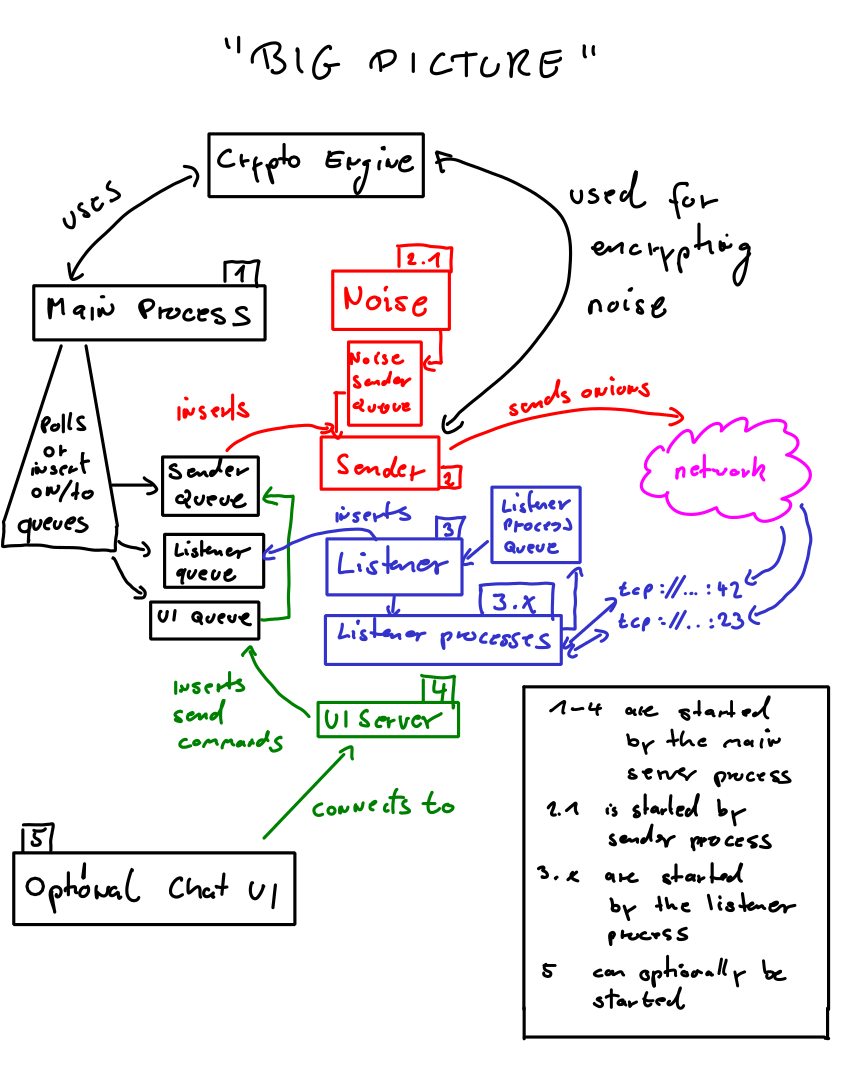
\includegraphics[scale=0.8]{bigpicture.png}
\end{figure}
As can be seen further in this figure, the processes communicate with
each other using queues. The optional chat user interface is also
integrated using a separate UIServer process.
% ----------------------------------------------------------------------------
\subsection{Sequence Numbers}
Sequence numbers for packets are encoded in a custom base 64 encoding to
define the used characters. Sequence numbers are stored in the
ID field (section \ref{eofid}) and can range from 0 to 68719476735 ($(64^6)-1$).

The transformation from an integer to an sequence 
number (also called \textit{eofid}) is made based on transformation
of a string and indexes. The \textit{get\_next()} method returns
the next sequence number and takes care of range overflows.
Code parts are show in figure \ref{eofidexample}.
\begin{figure}[htbp]
\caption{EOFID Code Example}
\label{eofidexample}
\begin{verbatim}
...
EOF_ID_CHARS = "0123456789abcdefghijklmnopqrstuvwxyzABCDEFGHIJKLMNOPQRSTUVWXYZ-!"
...

    def int_to_id(to_convert):
        """Convert int to ID"""
        index = ceof.EOF_L_ID-1
        eofid = []

        while index >= 0:
            part = ceof.EOF_ID_BASE**index

            # Fits in? Record and subtract
            if (to_convert - part) >= 0:
                times = int(to_convert / part)
                to_convert = to_convert - (times*part)
            else:
                times = 0 

            # Append selected symbol
            eofid.append(ceof.EOF_ID_CHARS[times])
            index = index - 1 

        return "".join(eofid)
\end{verbatim}
\end{figure}
% ----------------------------------------------------------------------------
\subsection{Queuing}
Several queues have been implemented for use of 
\textit{inter process communication (IPC)} as shown in figure \ref{bigpicture}.
The main server process creates queues on startup and polls them regularly.
As it is not clear, whether using the \textit{select()} method
for polling is interoperable, manual polling with a sleep timeout has been 
implemented. The queue and polling process
has been programmed generic, so the main server can use one loop
to poll data on all queues and selects the right handler based on
a dictionary entry, which has the same name as the queue dictionary
entry (figure \ref{queuepoll}).
\begin{figure}[htbp]
\caption{Queues / Polling Code Example}
\label{queuepoll}
\begin{verbatim}
        while True:
            for name, q in self.queue.items():
                log.debug("Polling on %s queue" % name)
                data = False
                try:
                    data = q.get(block=False)
                except queue.Empty:
                    pass

                if data:
                    log.debug("Got message from: %s:%s" % (name, data))
                    self.handler[name](data)

            time.sleep(ceof.EOF_TIME_QPOLL)
\end{verbatim}
\end{figure}
% ----------------------------------------------------------------------------
\subsection{Onion Creation}
To support onion routing, the sender of a messages needs to encrypt the packet
multiple times, once for each host that receives the packet. 
The process to do so may look like this:
\begin{enumerate}
\item Create message (from noise or user input)
\item Create source path
\item Create packet for last peer
\item Create packet for last-1 peer including previous packet
\item Continue until first peer is reached
\item Sent packet to first peer 
\end{enumerate}
The actual implementation can be found in \textit{src/lib/ceof/onion.py}.
An excerpt on how the onion is created can be seen in figure \ref{onionexample}.
\begin{figure}[htbp]
\caption{Onion Example Code}
\label{onionexample}
\begin{verbatim}
...
# Initialise parameters
                peer = ceof.Peer.from_disk(config.peer_dir, args.name)
                route = ceof.TransportProtocol.route_to(config.peer_dir, 
                    peer, ceof.EOF_L_ADDITIONAL_PEERS)
                chain = ceof.TransportProtocol.chain_to(route, peer, args.message)
                # Copy for debug
                orig_chain = list(chain)

                onion = cls(config.gpg_config_dir)
                onion_chain = onion.chain(chain)
...
    def chain(self, chain):
        """Create an onion chain"""

        # Get our packet to work on
        pkg = chain.pop()
        log.debug("Onion: Encrypting for %s, chain = %s" % (str(pkg), str(chain)))

        # If there is more, call us again
        if chain:
            inner_part = self.chain(chain)
        else:   
            inner_part = ""

        eofmsg = pkg['eofmsg']
        fingerprint = pkg['peer'].fingerprint

        onion = self.crypto.encrypt(str(eofmsg) + str(inner_part), fingerprint)

        return str(onion)
\end{verbatim}
\end{figure}
% ----------------------------------------------------------------------------
\section{Test of the Prototype}
%    6. Description of test results
Several tests were made to verify the correct behaviour of the prototype.
For most tests the network sniffer Wireshark was used to verify what can be
seen on the wire.
% ----------------------------------------------------------------------------
\subsection{Onion Structure}
This test verifies that an onion is constructed in the correct order and that
the correct fields being setup and noisified for every peer.
This test was done by running the implementation with the following
parameters:\\ \verb=./bin/ceof onion --plain --debug --message Test peer0=.
After analysing the output, it was verified that the onion is created in the
correct order and fields contain noise.
\subsubsection{Test Result}
\begin{itemize}
\item Success
\end{itemize}
% ----------------------------------------------------------------------------
\subsection{Noise Sending}
\label{testnoisesending}
This objective of this test is to verify that the implementation
\begin{enumerate}[(a)]
\item sends out packets regularly 
\item selects different destination peers
\item selects different addresses of each peer
\end{enumerate}
\subsubsection{Test Setup}
The implementation was configured to know about 11 peers,
with each one having at least two addresses in the format
of \verb=tcp://127.0.0.1:4294=, where the port was a random
port in the range of 4000-50000.
The implementation was started using
\\ \verb=./bin/ceof server --verbose=. The packets
on the network were captured using the network sniffer.
To be able to receive the packets, the \textit{socat} command was started
to listen on all ports on which the peers would listen. The
socat command line is shown in figure \ref{socatlisten}.
\begin{figure}[htbp]
\caption{Socat command line for testing}
\label{socatlisten}
\begin{verbatim}
for port in $(cat ~/.ceof/peers/*/addresses | sed 's/.*://'); do
    ( socat TCP4-LISTEN:$port,reuseaddr,fork - & );
done
\end{verbatim}
\end{figure}
\subsubsection{Test Result}
\begin{itemize}
\item Success
\end{itemize}
Using the timeline of the network sniffer and a filter
to match only new packets
(\textit{tcp.flags.syn == 1 and tcp.flags.ack == 0}),
it was revealed that the sending interval equals to
the one defined in the chat protocol. 
To verify that all related component of the
implementation depend on the specific internal sending
interval, the sending interval was changed from 
\textbf{0.250s} to \textbf{0.125s}. 
The difference on the network traffic can be seen in figures
\ref{sending0250} and \ref{sending0125}.
\begin{figure}[htbp]
\caption{Sending data at 0.250s interval}
\label{sending0250}
\centering
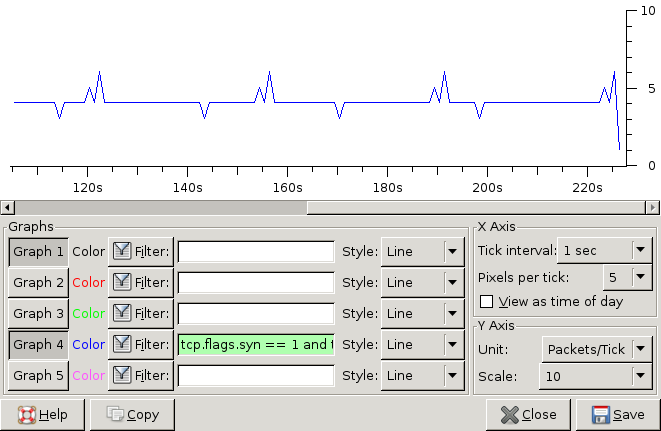
\includegraphics[scale=0.5]{noise-at-0250s.png}
\end{figure}
\begin{figure}[htbp]
\caption{Sending data at 0.125s interval}
\label{sending0125}
\centering
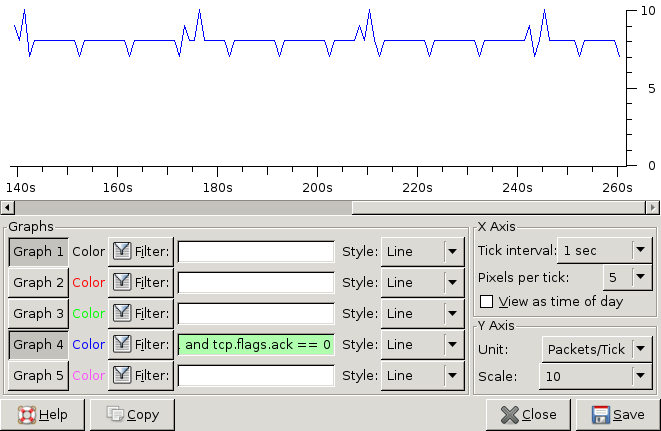
\includegraphics[scale=0.5]{noise-at-0125s.png}
\end{figure}
The selected destination addresses as seen in the network
sniffer were compared with the addresses of the peers to verify
that the implementation does indeed select different peers
and different addresses of each peer.
% ----------------------------------------------------------------------------
\subsection{Encryption}
\label{testencryption}
This test is used to verify that all network traffic is encrypted.
% \begin{enumerate}[(a)]
% \item real messages
% \item and noise
% \end{enumerate}
%% \begin{enumerate}
%% \item is encrypted
%% \item cannot be distinguished from each other
%% \end{enumerate}
\subsubsection{Test Setup}
The setup was prepared identical to the one described
in section \ref{testnoisesending}. All packets seen within
an interval of 60 seconds, in the network sniffer and on 
the receiving side, were analysed.
\subsubsection{Test Result}
\begin{itemize}
\item Success
\end{itemize}
All encrypted messages have been filtered out of the captured
packet list. Zero packets have been left, no unencrypted traffic
was produced by the implementation.
% ----------------------------------------------------------------------------
\subsection{Receiving Peers Can Decrypt Message}
When sending out a message to another peer, the message should
be decrypt-able and readable by the receiving peer, independent of the
message type. This test verifies that messages can be decrypted.
\subsubsection{Test Setup}
In contrast to the tests described in sections
\ref{testnoisesending} and \ref{testencryption}, only
one postcard was produced. The number of known peers was shrunk
to \textbf{6}, so that every participant needs to receive a postcard.
Afterwards a test instance for every peer was started using
the script \verb=start_peers.sh= (see \ref{scriptstartpeers}, p.
\pageref{scriptstartpeers}).
Afterwards a message was sent manually using
\\ \verb=./bin/ceof onion -m "hallo peer0" -s peer0=.
\subsubsection{Test Result}
\begin{itemize}
\item Success
\end{itemize}
As can be seen in the log files of each implementation,
the message was received by all peers and successfully decrypted,
displayed (in case of \textit{peer0}) and forwarded until the last
peer.
% ----------------------------------------------------------------------------
\subsection{Receiving Peer: Authenticity Verification}
When sending out a real message to another peer, the message should be
encrypted and signed. 
The current prototype does \textbf{not} contain
the logic to sign messages nor to verify signatures.
\subsubsection{Test Result}
\begin{itemize}
\item Fail
\end{itemize}
% ----------------------------------------------------------------------------
\subsection{Effective Bandwidth Usage}
The calculations in section \ref{bandwidthusage} are based on experimental
packet sizes as seen in section \ref{pkgsizes}, which do not include
protocol overhead. This test should reveal the effective required
bandwidth.
\subsubsection{Test Setup}
To test the effective bandwidth usage three steps are taken:
\begin{itemize}
\item Measure idle bandwidth (a)
\item Measure bandwidth while running the prototype (b)
\item Calculate effective bandwidth as a difference of b and a
\end{itemize}
To simplify the test, it was ensured that the idle bandwidth on the
loopback interface was 0 Bit per second.
The setup was prepared identical to the one described
in section \ref{testnoisesending}, with additionally changing
the sending interval to the values \textbf{0.125s},
\textbf{0.250s} and \textbf{0.500s}.
\subsubsection{Test Result}
When sending packets at the defined interval of
\textbf{0.250s}, the effective bandwidth measured is
circa 25000 Bytes (24 KiB) per second.
When changing the interval to \textbf{0.500s},
the effective bandwidth measured is
12000 Bytes (12 KiB) per second, when changed
to \textbf{0.125s}, it is 50000 Bytes (49KiB) per second.
Figures \ref{bw0125}, \ref{bw0250} and
\ref{bw0500} show the test results from the network sniffer.
Comparing these numbers to the calculated bandwidth usage
(section \ref{bwusagetheory}, p. \pageref{bwusagetheory}),
the effective bandwidth usage is 1.5 times higher than 
calculated ($50000 / 32768 = 1.52587890625$, $25000 / 16384 = 1.52587890625$,
12000 / 8000 = 1.5). Thus, the measured bandwidth of 24 KiB/s or
192 KBit/s is the required outgoing bandwidth to run the chat system.
\begin{figure}[htbp]
\caption{Effective Bandwidth Usage (0.125s)}
\label{bw0125}
\centering
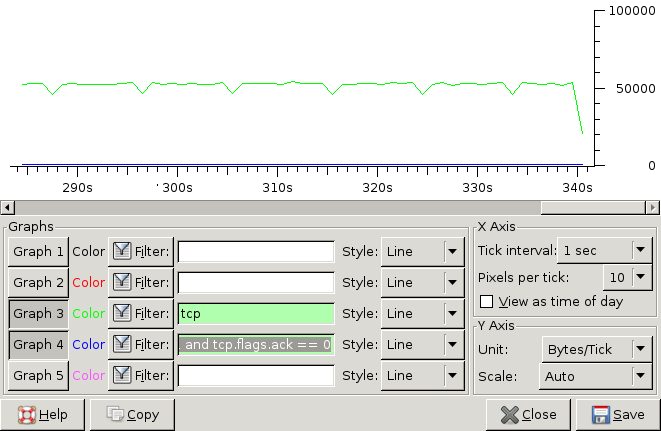
\includegraphics[scale=0.5]{bandwidth-0125.png}
\end{figure}
\begin{figure}[htbp]
\caption{Effective Bandwidth Usage (0.250s)}
\label{bw0250}
\centering
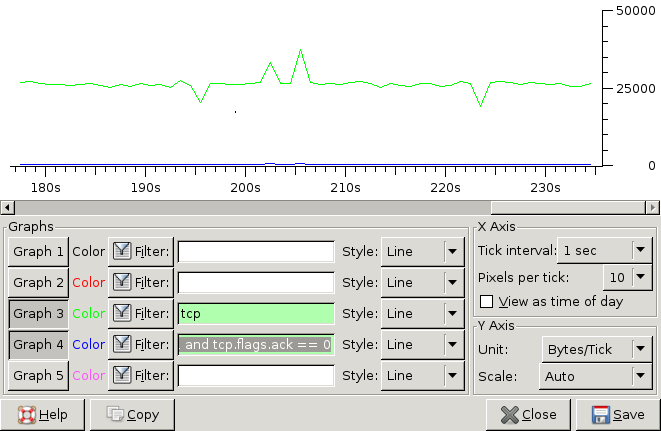
\includegraphics[scale=0.5]{bandwidth-0250.png}
\end{figure}
\begin{figure}[htbp]
\caption{Effective Bandwidth Usage (0.500s)}
\label{bw0500}
\centering
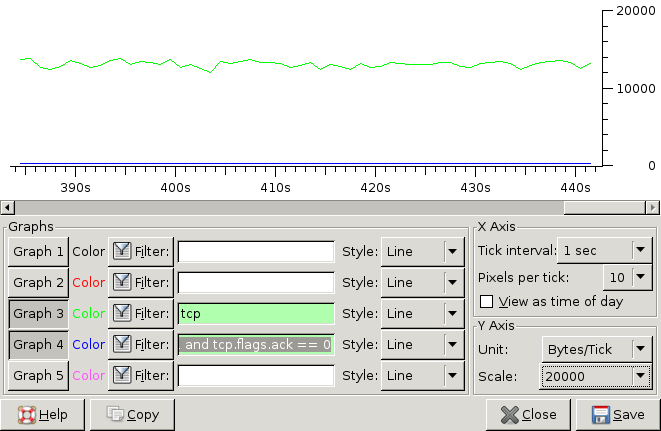
\includegraphics[scale=0.5]{bandwidth-0500.png}
\end{figure}
% ----------------------------------------------------------------------------
\subsection{Performance}
It is important that the system generating noise is able to generate 
and send noise at the given interval of \textbf{0.25s}.
\subsubsection{Test Setup}
This test was inverted and instead of trying to send out data
at an interval of \textbf{0.25s}, the artificial sending limit was removed
and measured how many packets per second could be send.
The setup was prepared identical to the one described
in section \ref{testnoisesending}. 
\subsubsection{Test Result}
\begin{itemize}
\item Success
\end{itemize}
When sending without a limit, a maximum of 13 packets / second
was measured (see figure \{noisenolimit). The CPU
usage of one core was around 38\% during the test.
\begin{figure}[htbp]
\caption{Packets per second (without sending limit)}
\label{noisenolimit}
\centering
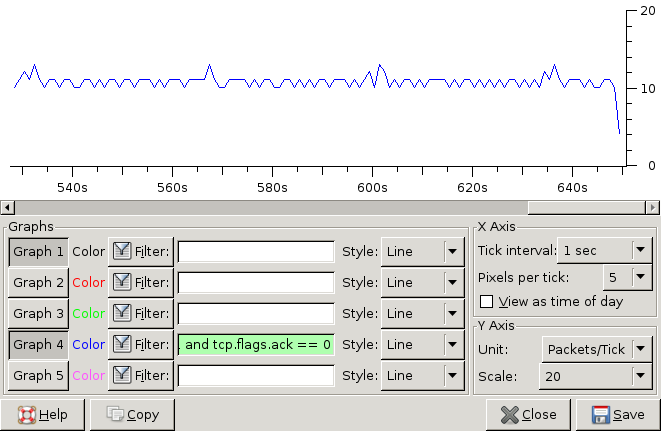
\includegraphics[scale=0.5]{noise-no-limit.png}
\end{figure}
As the encryption was suspected to limit the number
of outgoing packets, another test with plain text
packets (i.e. no encryption) was made.
When changing the implementation to send out 
plain text packets instead of onions the
CPU usage raised to 100\% and
around 250 packets / second were sent (see figure
\ref{noisenolimitplain}.
\begin{figure}[htbp]
\caption{Packets per second (without sending limit, plain text)}
\label{noisenolimitplain}
\centering
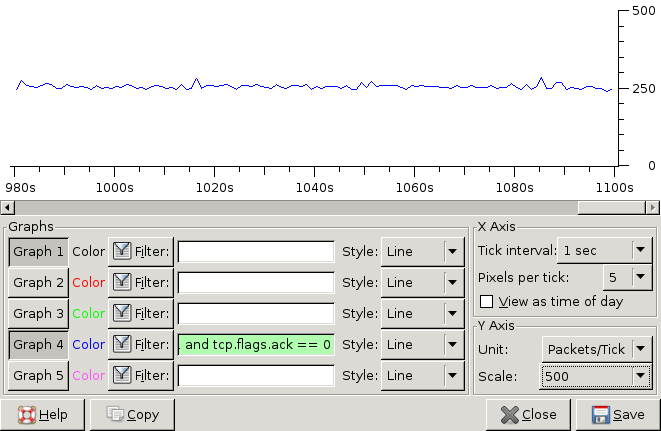
\includegraphics[scale=0.5]{noise-plain-no-limit.png}
\end{figure}
% ----------------------------------------------------------------------------
\section{Features}
Based on the requirements defined in section \ref{protofeatures}, 
p. \pageref{protofeatures}, the following features have been implemented. 
% ----------------------------------------------------------------------------
\subsection{Anonymity}
The existing prototype implements anonymity including
all features as described in section \ref{featanonymity}.
Currently the number of proxy peers is hardcoded to 5. This implementation
limit can easily be changed and made a command line parameter.
%Before the encrypt the packet, it is signed via public-key
%cryptography\cite{pgp-1}. Thus only the receiver can verify the message sender.
%% We don't think it's possible to hide that you are part of the chat network,
%% because some heuristics will be developed to detect the chat packets.
%% So we use a different idea:
%% Every participant of an EOF network will constantly send chat packets
%% with a pre-defined frequency (for instance every 250 ms). 
%% If you don't chat, \emph{noise} is sent.\footnote{Noise is just random
%% data, see below for a more detailled description of noise.}
%% The noise is also used to defend against timing analysis.
%% In case you are sending out a message, the message packet will be added to the
%% queue and sent within the next free time slot.
%% 
%% From outside it can easily be seen, that you are part of the network,
%% but not, if you sent a message.
% ----------------------------------------------------------------------------
\subsection{Authenticity and Confidentiality}
The prototype does not sign messages and thus the authenticity is not
verifiable. It does encrypt the messages multiple times, though.
Adding authenticity requires two modifications to the source code:
\begin{itemize}
\item Sign real messages (EOFmsg 3002 / 3003)
\item Check signature on real messages
\end{itemize}
Integrity checking can be done with any signed messages, sender verification
is only possible for messages which have been signed with a reasonable
trusted public key. As this includes the implementation of trustlevels, the
prototype does not support authenticity verification.
% ----------------------------------------------------------------------------
\subsection{Availability}
Availability should be provided by
\begin{itemize}
\item Transport protocol multiplexing (\ref{multiplexing}, p. \pageref{multiplexing})
\item Transport protocol tunnelling (\ref{tunneling}, p. \pageref{tunneling})
\end{itemize}
The current prototype supports only one transport protocol, but allows to listen on
a number of tcp ports. Thus the onions are encoded and tunnelled only into
one transport protocol. The source code allows to seamless integrate a new
transport protocol, by creating a new folder below
\textit{src/lib/ceof/tp/} with the name of the transport protocol and adding
a python module into it. The existing implementation of tcp can be used
as an example.
%% \subsubsection{Reliable against single user attacks}
%% Traditional chat networks depend on one or more central organised servers.
%% An attacker can stop all communication, if she runs a successful denial
%% of service ("`DoS"') attack against the central systems.
%% To protect against this, EOF uses a dynamic peer-to-peer network, which works
%% as long as the minimun number of peers and the destination peer is available.
%% It has no dependency on a central server.
%% 
%% \subsubsection{Hide packets in network stream}
%% As said before, we don't think it's possible to hide the participation in the
%% chat network. To be able to send packets, although an attacker \emph{knows}
%% about the participation, EOF embeds all chat packets into other (well known)
%% protocols (which is knows as steganography\cite{stegano-1}).
%% EOF does not implement nor specify \emph{transport protocols} itself.
%% The EOF community is urged to implement them in a creative way: Usage
%% of well-known protocols like TCP\cite{tcp-1}, HTTP\cite{http-1},
%% SMTP\cite{smtp-1} or even transmission of packets on avian
%% carriers\cite{avian-1} are encouraged. The tunneling of EOF packets through
%% those protocols (also know as obfuscation) makes it harder to detect
%% and \emph{block} EOF traffic. 
%% If an attacker wants you to stop sending messages, she has to completly
%% remove you from the network, because any open protocol may be (ab)used to
%% encapsulate EOF packets into it.
%% % Nico: 1.0 
% ----------------------------------------------------------------------------
\section{Related Project: Chat User Interface}
\label{chatui}
In addition to the described prototype, in a different
project a chat user interfaces has been
developed that can talk to the prototype using a chat server.
This chat UI is documented in the file \textit{doc/appendix/chat-ui.pdf},
which is included in the digital distribution.
